
\chapter[Renderización de la geometría de Panes]{Renderización de la geometría de Panes y otros Materiales Porosos}
\section{Introducción}
Debido a las limitaciones existentes actualmente en el renderizado realista de pan, nos proponemos en este capítulo estudiar la utilización de renderizado directo de volúmenes aplicado a un campo escalar representando la geometría de la miga de pan. 

Los resultados obtenidos son realistas y se renderizan en tiempo real. La misma evita el uso de estructuras intermedias, simplificando el desarrollo y reduciendo los costos computacionales.
El renderizado foto-realístico de materiales con una estructura interna compleja presenta grandes retos en Computación Gráfica.
En particular, las migas de panes son un material translúcido complejo, con una estructura porosa, que presenta detalles diferentes en distintas escalas, todos igualmente necesarios de ser tenidos en cuenta para lograr una correcta visualización.
El renderizado realista de estos materiales debe simular correctamente diversos fenómenos como translucencia, auto-sombreado, auto-oclusión, reflectancia, y absorción, entre otros.

Las técnicas del estado del arte en renderizado de migas de panes tratan el material como una superficie, seteando un complejo procedimiento de captura, en el cual la luz reflejada por el material es fotografiada en distintos ángulos.
Luego, la información es procesada y reconstruída para formar un modelo del material.
Si bien esta solución es capaz de capturar los fenómenos lumínicos previamente discutidos, también es cierto que la practicidad del método está severamente comprometida, ya que presenta un costo computacional alto, un procedimiento de captura muy limitado y la imposibilidad de obtener más de una apariencia con una única captura.

En un intento por superar estas limitaciones del renderizado, proponemos, en conjunción con el capítulo anterior de modelado de la geometría, utilizar un modelo volumétrico del pan.
Para esto utilizamos la técnica de renderizado directo de volúmenes, implementada en GPU.
La técnica permite renderizar los campos escalares del capítulo anterior sin utilizar estructuras intermedias.
Las imágenes obtenidas son promisorias, y se computan en tiempo real gracias al poder de las placas gráficas actuales.

%La inmensa variedad de materiales y su compleja interacción con la luz han sido un tópico central en computación gráfica por décadas.
%El modelado de materiales en física ha obtenido resultados excelentes en fenómenos relacionados con el transporte de la luz. Las aproximaciones computacionales a estos fenómenos son, actualmente, sujeto de gran interés en el renderizado en computación gráfica.
%En materiales complejos, el modelado de la geometría de los mismos sigue una estrategia de investigación similar, comenzando con una comprensión física del material, la cual luego se aproximará computacionalmente.

%Finalmente, una representación computacional realista del material debe tener en cuenta tanto el modelado geométrico como la interacción de la luz, simultáneamente.



%The method obtains very promising images in real time.

\section{Trabajo Previo}
El tópico de renderizado foto-realista de materiales, y su modelado, atrajo un interés creciente en la literatura científica.
La mayoría de los esfuerzos están focalizados en materiales complejos de frecuente aparición como el agua \cite{Schechter2012}, la piel humana \cite{Donner2006}, metales, plásticos \cite{Kurt2010}, etc.
La comunidad de investigadores, sin embargo, ha tenido grandes dificultades para simular adecuadamente la apariencia de otros materiales, como es el caso de materiales cocidos ({\em e.g.}, pizza, galletitas).
Debido a su compleja geometría y fenómenos lumínicos involucrados, esto continúa siendo un problema abierto \cite{Voglsam2013}.

Hasta hace pocos años, el costo computacional de renderizar modelos físicos de estos materiales resultaba prohibitivo si el tiempo real era un requerimiento.
De todas formas, el crecimiento notable en poder de cómputo debido al diseño masivamente paralelo de las placas gráficas \cite{Yeo09,Harris06}, está permitiendo la simulación de complejos fenómenos de interacción de la luz con los materiales en tiempos de cómputo aceptables.

Simular un modelo geométrico aceptable representa un reto adicional, como fue visto en el capítulo anterior.
El pan y otras estructuras porosas con el resultado de mecanismos complejos que involucran deformaciones físicas, transferencia de masa y calor durante la cocción, y distintas reacciones químicas.

Estudios recientes utilizan consideraciones fenomenológicas sobre panes reales, pero la geometría es invariable ({\em i.e.}, no es procedimental) \cite{VanDyck2014}: una geometría fija no permite obtener diferentes tipos de pan fácilmente, ya que requiere un procedimiento de captura para cada uno de ellos.
Adicionalmente, las distribuciones de burbujas no pueden ser controladas.

La presencia de mesoestructuras (burbujas con formas complejas) hacen del pan un material {\em quasi-homogéneo} \cite{Tong2005}. 
Por esta razón, modelar al material como una superficie no resulta adecuado.
Técnicas típicas como funciones bidireccionales de distribución de reflectancia (BRDF en inglés) \cite{Kurt2009}, y funciones bidireccionales de distribución de reflectancia y translucencia (BSSRDF en inglés) \cite{Donner2009}, no resultan satisfactorias.
Una publicación intenta resolver las limitaciones \cite{Tong2005}, pero las desventajas que acarrea (proceso de captura muy complejo, altos costos computacionales, invariabilidad geométrica), resultan en un proceso muy poco práctico.

Por otro lado, es común encontrar procesos físicamente inspirados sobre modelado de distintas etapas del proceso de formación del pan en la literatura de ingeniería de los alimentos.
Estos trabajos modelan las distribuciones de calor y masa en panes durante la cocción, entre otros fenómenos.
Recientemente, determinados resultados sugieren que estos objetivos pueden ser alcanzados utilizando modelos unidimensionales.
Por ejemplo, modelar la geometría como un cilindro infinito, o asumir una única coordenada radial \cite{Purlis2012, Thorvaldsson1999}.

Estos y otros resultados en la industria de los alimentos tienen cierta significancia en el modelado y la renderización de geometrías de panes, y pueden ser usado como base para futuros modelos computacionales de la cocción del pan.


\section{Renderizado Directo de Volúmenes (DVR)}

La técnica de renderizado directo de volúmenes (DVR) \cite{Kratz2006} gebera imágenes bidimensionales computando la interacción de la luz con un medio semi-transparente, el cual es representado con un campo escalar discreto.
Este campo describe la densidad del medio en cada celda discretizada.
Para cada píxel en la imagen, se computa un rayo desde la posición de la cámara en el espacio virtual, y la radiancia que alcanza la cámara desde esa dirección es computada aproximando la ecuación del transporte radiativo (RTE en inglés).
Esta ecuación describe el cambio en radiancia a medida que el rayo atraviesa el medio no transparente.

En su forma completa, la RTE incorpora muchas propiedades ópiticas y efectos.
Para aproximar el resultado de la RTE en tiempo real, este capítulo utiliza una versión simplificada de la ecuación que sólo toma en consideración algunos de los fenómenos ópticos que ocurren en la realidad.

Existen tres fenómenos ópticos importantes que afectan la propagación de la luz a través de un medio en un punto dado del espacio: emisión, absorción, y dispersión.
Emisión es la generación de energía radiante en una dirección dada.
La Absorción ocurre cuando una fracción o toda la energía radiante en el rayo de luz se topa con un objeto opaco y es transformada en otras formas de energía.

Finalmente, la dispersión produce cambios de dirección en los fotones.
Aquellos eventos que provocan que los fotones cambien su dirección a otra distinta a la dirección del rayo, son llamados de dispersión saliente. Del mismo modo, los eventos que provocan que los fotones cambien su dirección por la del rayo actual se llaman dispersión entrante.

%
La contribución de la dispersión entrante en la radiancia es computada a partir de una única dirección, la cual corresponde a la principal fuente de luz de la escena.
Esto aproxima la energía radiativa que llega a un punto desde la fuente de luz, haciendo rebotar a las partículas en el medio hacia ese punto y luego viajando a lo largo de una dirección dada. 

La RTE puede sintetizarse como sigue,

\begin{equation} \label{eq:general_radiance}  
  L(p_n) = L_b + \int_{p_0}^{p_n} \frac{\partial L(t)}{\partial p} \, dt,
\end{equation}

\noindent donde $L_b$ es la radiancia de fondo, y $p_0$, $p_n$ son los puntos visibles más cercano y más lejano en la dirección del rayo, respectivamente, $L(t)$  es la radiancia en el punto $t$, y $\partial p$ es la distancia entre puntos consecutivos muestreados. 
Debido a que la entrada del algoritmo de DVR es un conjunto de datos discreto, para computar $L(p_n)$ la integral es aproximada por una suma.

La extinción es el descenso en radiancia en un rayo debido a absorción y dispersión saliente.
Podemos aproximar este efecto definiendo un coeficiente de absorción para el medio, $k_a$ y un coeficiente de dispersión saliente $k_s$. 
Si descartamos el efecto de dispersión saliente, la fórmula que describe la radiancia alcanzando un punto luego de atravesar un segmento de un rayo es:

\begin{equation} \label{eq:radiance_absorption}  
    L_b \ e^{- \textstyle  \int_{p_0}^{p_n} k_a(t) \, dt}.
\end{equation}

Introducimos el valor $\int_{p_i}^{p_j} k_a(t) \, dt$, el coeficiente de absorción, el cual referiremos como $\tau_{(p_i, p_j)}$. 
La transmitancia es el concepto complementario a la extinción. Describe la cantidad de luz que pasa a través de un medio en una dirección dada.
Por lo tanto, el valor de la transmitancia entre dos puntos $p_i$ y $p_j$ es:

\begin{equation} \label{eq:transmittance}  
  T(p_i,p_j) = e^{- \textstyle \tau_{(p_i, p_j)}}.
\end{equation}

Si asumimos que en cada punto del rayo dentro del volumen existe un incremento en la radiancia, dada por dispersión entrante y fenómenos emisión ($\rho$), luego nuestra estimación inicial de radiancia resulta,

\begin{equation} \label{eq:ray_radiance}  
  L(p_n) = L_b \ e^{-\tau(p_0, p_n)} + \int_{p_0}^{p_n} \rho \ e^{-\tau(t,p_n)} \, dt.
\end{equation}

Esto significa que la radiancia a lo largo de los puntos $p_0$ y $p_n$ es la radiancia de fondo atenuada, más la emisión y la dispersión entrante atenuadas en cada punto del rayo.

El algoritmo de DVR muestrea la función de densidad del volumen a intervalos regulares, aproxima la transmitancia a lo largo de esos puntos y computa la cantidad de luz que llega a la cámara a lo largo de la dirección del rayo.
La computación reemplaza la suma integral por una suma discreta sobre el rayo intersectando el volumen,

\begin{equation} \label{eq:ray_radiance}  
  L(p_n) = L_b \ e^{-\tau(p_0, p_n)} + \sum_{p_0}^{p_n} \rho \ e^{-\tau(p_i,p_n)}.
\end{equation}

Es posible tener en cuenta otros efectos, aumentando la fidelidad de la imagen final, así como los costos computacionales de la técnica.
La base de nuestro algoritmo de renderizado utiliza un modelo simplificado que sólo tiene en cuenta transmitancia y emisión, junto con ciertas consideraciones artísticas, para alcanzar tasas de refresco de tiempo real.
Describiremos el algoritmo de renderizado en detalle en una sección posterior.

%~\ref{sec:rendering}.
%%%%%%%%%%%%%%%%%%%%%%%%%%%%
%La técnica de DVR tiene como objetivo crear una representación bidimensional de un volumen
%definido por una función de densidad tridimensiopocnal. Para ello, se emiten rayos desde el punto de vista de una cámara en una escena virtual y se utiliza la función de densidad para calcular la cantidad de luz que la cámara recibe en la dirección del rayo. Para esto se evalúa la función de densidad en el camino del rayo y se usan los valores adquiridos para aproximar el efecto de varios fenómenos lumínicos, como pueden ser la extinción, transmitancia, o dispersión lumínica, entre otros. La información obtenida de procesar todos los rayos se utiliza para definir el color de los pixeles en la imagen final.

%La radiancia es la cantidad de luz que pasa, o es emitida, desde un punto y atraviesa un determinado ángulo sólido. En el contexto de DVR, el medio que los rayos atraviesan, y que es definido por una función de densidad, es considerado como emisivo. Por lo tanto, cuando se busca calcular la cantidad de luz recibida en la dirección de un rayo, lo que se hace es aproximar la radiancia recibida de un punto distante siguiendo la dirección del rayo. El valor de la radiancia es aproximado como la suma de una radiancia de fondo y la radiancia emitida por el medio por el cuál se mueve el rayo \cite{Kratz2006} :

%\begin{equation} \label{eq:general_radiance}  
%  L(p_n) = L_b + \int_{p_0}^{p_n} \frac{\partial L(t)}{\partial p} \, dt,
%\end{equation}

%\noindent donde $L_b$ es la radiancia de fondo, $p_0$ y $p_n$ son los puntos inspeccionados en la dirección del rayo más cercano y más lejano respectivamente, $L(t)$ es la radiancia evaluada en el punto $t$, y $\partial p$ es la distancia entre puntos evaluados. En el momento de calcular $L(p_n)$, la integral es aproximada por una suma.

%La extinción es la pérdida de fotones en un haz de luz debido a la absorción en el medio que atraviesa y la dispersión hacia otras direcciones. Algunos de los fotones colisionarán con particulas del medio y serán absorbidas y transformadas en otras formas de energía, mayormente calor. Otras rebotarán y pasarán a moverse en otras direcciones. Estos fenómenos se aproximan usando un coeficiente de absorción para el medio, $k_a$ y un coeficiente de dispersión $k_s$. Si el efecto de dispersión es ignorado, la fórmula que define la cantidad de radiancia absorbida en el largo de un segmento de rayo
%es: 

%\begin{equation} \label{eq:radiance_absorption}  
%    L_b \ e^{- \textstyle  \int_{p_0}^{p_n} k_a(t) \, dt}.
%\end{equation}

%El valor $\int_{p_i}^{p_j} k_a(t) \, dt$ es llamado coeficiente de absorción y se referenciar\'a como $\tau_{(p_i, p_j)}$.

%La transmitancia es un concepto complementario a la extinción y describe la cantidad de luz que pasa por un medio en una dirección determinada. El valor de transmitancia entre dos puntos $p_i$ y $p_j$
%es:

%\begin{equation} \label{eq:general_radiance}  
%  T(p_i,p_j) = e^{- \textstyle \tau_{(p_i, p_j)}}.
%\end{equation}

%Si la emisión de luz se asume como un término constante ($\rho$) para todos los puntos del medio, la fórmula inicial de radiancia queda:

%\begin{equation} \label{eq:ray_radiance}  
%  L(p_n) = L_b \ e^{-\tau(p_0, p_n)} + \int_{p_0}^{p_n} \rho \ e^{-\tau(t,p_n)} \, dt.
%\end{equation}

%Esto significa que la radiancia entre los puntos $p_0$ y $p_n$ se puede calcular como la radiancia de fondo restante luego de la atenuación del medio sumada a la emisión, también atenuada, en todos los puntos del medio que atraviesa el rayo.

%La técnica de DVR define un volumen donde una función de densidad se evalúa en intervalos regulares y utiliza esa información para aproximar la transmitancia en esos puntos y de esa manera aproximar la cantidad de luz que llega a la cámara. La suma integral descrita anteriormente se reemplaza por una suma discreta de los puntos evaluados de un rayo donde \'este intersecta al volumen que interesa representar. 

%Otros efectos lumínicos pueden ser aproximados. Esto aumenta la fidelidad de la imagen final pero también aumenta el costo de cómputo de la técnica. Algunos de estos efectos son el cálculo de fase, el c\'alculo de luz entrante por dispersión o luz extinguida por dispersión, entre otros. Dado que el objetivo de este trabajo es lograr un renderizado en tiempo real, el algoritmo implementado usa como base el modelo de cálculo de radiancia simplificado que toma en cuenta sólo la
%transmitancia del medio.

\section{Implementación}

Se creó una aplicación demo \footnote{disponible en \emph{https://www.github.com/rbaravalle/Pysys}}  que usa el sistema de partículas descrito en secciones previas para renderizar panes en tiempo real, utilizando DVR.
La Fig.~\ref{fg:application} muestra la aplicación desarrollada, con un pan renderizado en tiempo real.


\begin{figure}
  \centerline{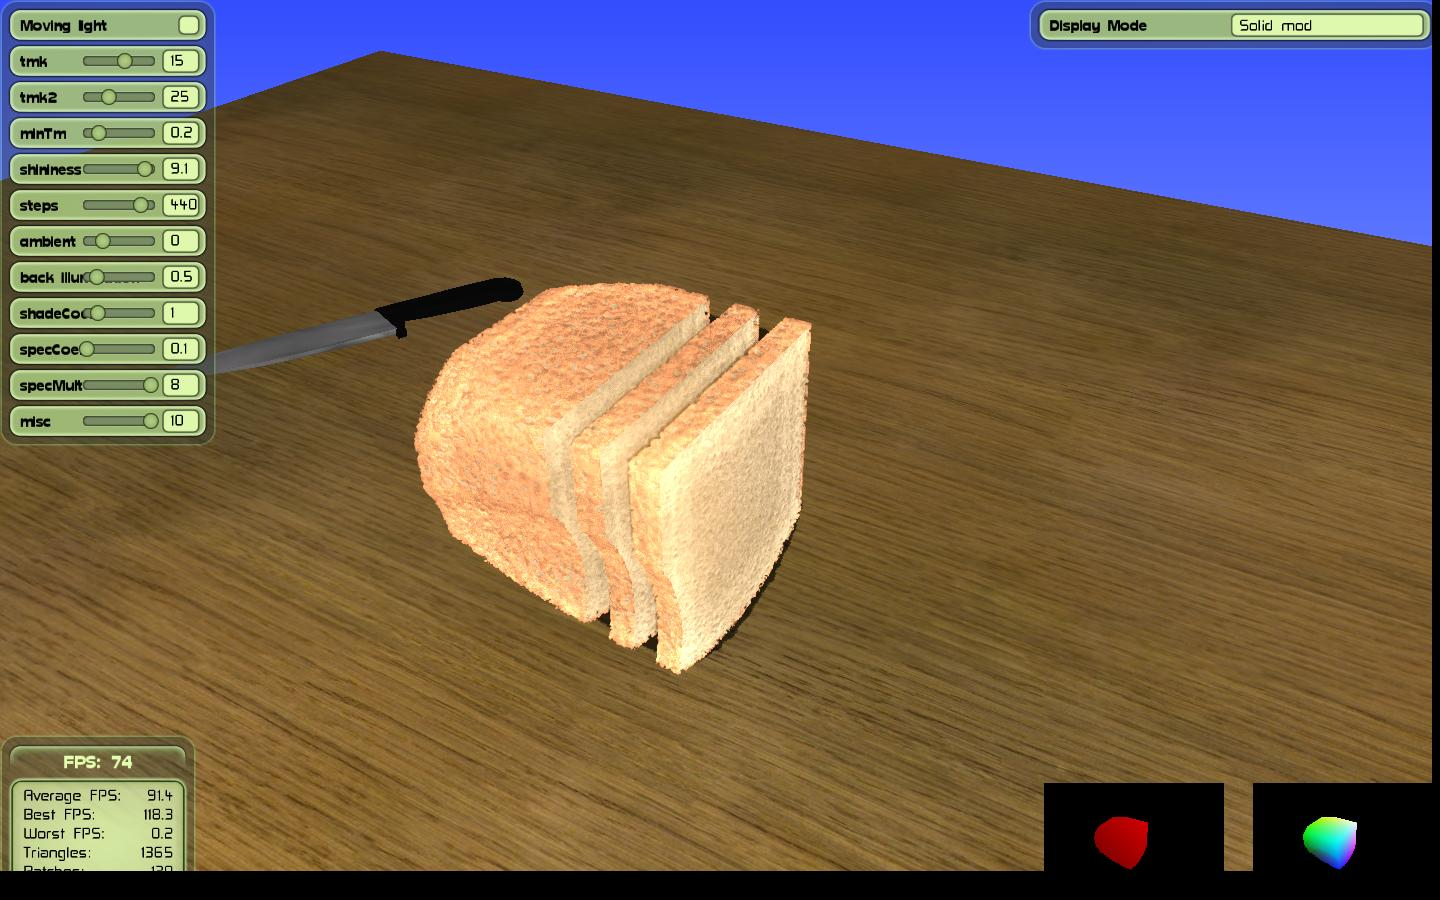
\includegraphics[width=13cm]{figures/application}}
  \caption{Aplicación desarrollada mostrando un pan renderizado en tiempo real.}
  \label{fg:application}
\end{figure}


En la demo, el SP descrito produce una textura volumétrica.
Un cubo que corresponde a esta textura es renderizado en la escena.
El material utilizado para renderizar el cubo consta de un shader de vértices muy simple, y un shader de fragmentos, el cual implementa el algoritmo de DVR.
Para cada fragmento, el shader computa un rayo con origen en la posición de la cámara y con la dirección del fragmento que debe ser coloreado.
El procedimiento muestrea la textura volumétrica a intervalos regulares sobre la intersección del rayo y el cubo.
Estos valores muestreados son luego utilizados como entrada de un algoritmo que implementa una versión simplificada de la RTE, computando el color del píxel resultante de la manera descrita en secciones previas.

En la implementación, estas ecuaciones acumulan la transmitancia del rayo y la contribución de radiancia en cada punto muestreado.
La computación termina si el valor de la transmitancia está por debajo un umbral o si el rayo sale del cubo.

La dispersión entrante, simplificada, se computa a través de un rayo secundario, para cada punto muestreado, en dirección a la fuente de luz.
Este rayo secundario es luego muestreado para determinar la cantidad de luz que llega al punto.
Esta técnica permite obtener sombras naturales dentro del volumen.

El píxel es sombreado utilizando la información de transmitancia del rayo primario y los secundarios en cada punto.
En este punto, diferentes consideraciones artísticas pueden ser aplicadas para obtener diferentes materiales con distintos aspectos.
Por ejemplo, podemos diferenciar miga de corteza asignando un coeficiente de extinción mayor y un color más oscuro a las regiones de corteza.
En nuestro caso, un color amarillo suave es aplicado en ciertas regiones, otorgándoles una apariencia de miga.
Adicionalmente se puede agregar una sutil reflexión especular.
Para esto, es necesario computar la primera intersección entre el rayo y el SP.
Gracias a esto se puede incrementar ligeramente el realismo final de la imagen.
El vector normal usado en este cálculo es el gradiente de la textura volumétrica en ese punto.

La demo presentada provee al usuario la habilidad de modificar parámetros como el coeficiente de transmitancia, el umbral de transmitancia, el color asignado a la miga y la visibilidad de los reflejos especulares.
Con la modificación de estos parámetros, el usuario puede producir imágenes que semejan otros materiales porosos como las esponjas.

\begin{figure*}[htb!]
  \centerline{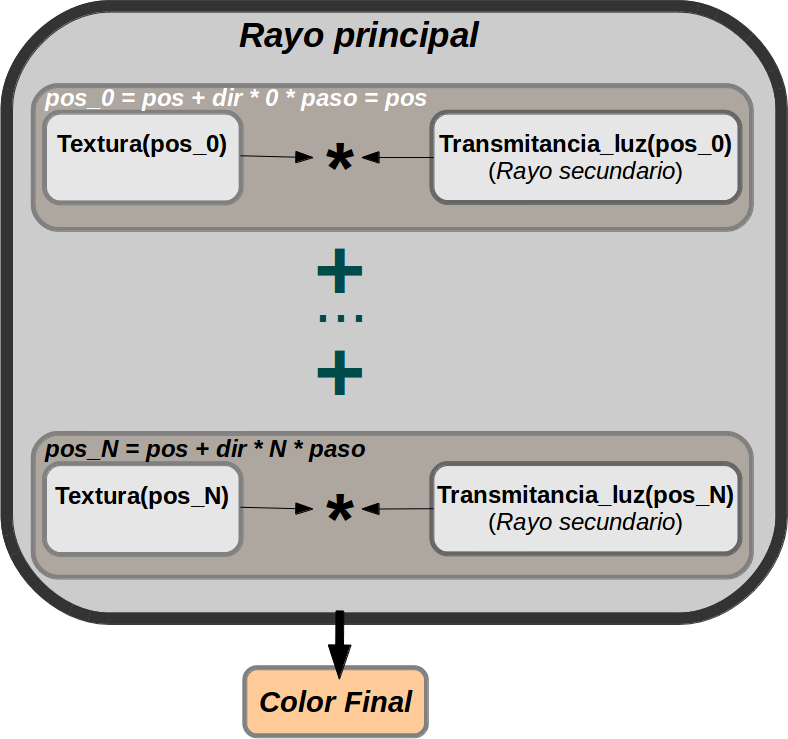
\includegraphics[width=13cm]{fragmentshader}}
  \caption{Cálculo de color en el shader de fragmentos. }
  \label{fg:fragmentshader}
\end{figure*}


\subsection{Oclusión Ambiente}

Un aspecto clave para resaltar la apariencia de la imagen final está basada en las contribuciones locales debido a características propias del material (emisión, oclusión, absorción).
La literatura muestra que considerar la oclusión del ambiente puede producir imágenes más realistas \cite{Hernell2010}.
Basados en esto, proponemos computar la dispersión entrante, múltiple, calculando de manera offline un término de oclusión del ambiente para cada voxel en el campo escalar y guardándolo como una textura volumétrica aparte, la cual es pasada al shader de fragmentos.

Para cada voxel, el cómputo de dicho término define un radio $r$ y guarda el valor medio de los vóxeles vecinos dentro de una esfera que contiene ese radio en la textura resultante del SP.
Luego, este valor se utiliza para modular la contribución de cada paso del rayo.
Experimentalmente encontramos que el valor $r$ resulta visualmente indistinguible al variarlo, por lo cual cualquier valor mayor que $0$ puede utilizarse para el cómputo.

La Fig.~\ref{fg:occlusion} muestra que el realce que produce este concepto no es despreciable, resultando en un aspecto clave de nuestra implementación, a la hora de producir imágenes creíbles de migas de pan. 



\begin{figure}
\centerline{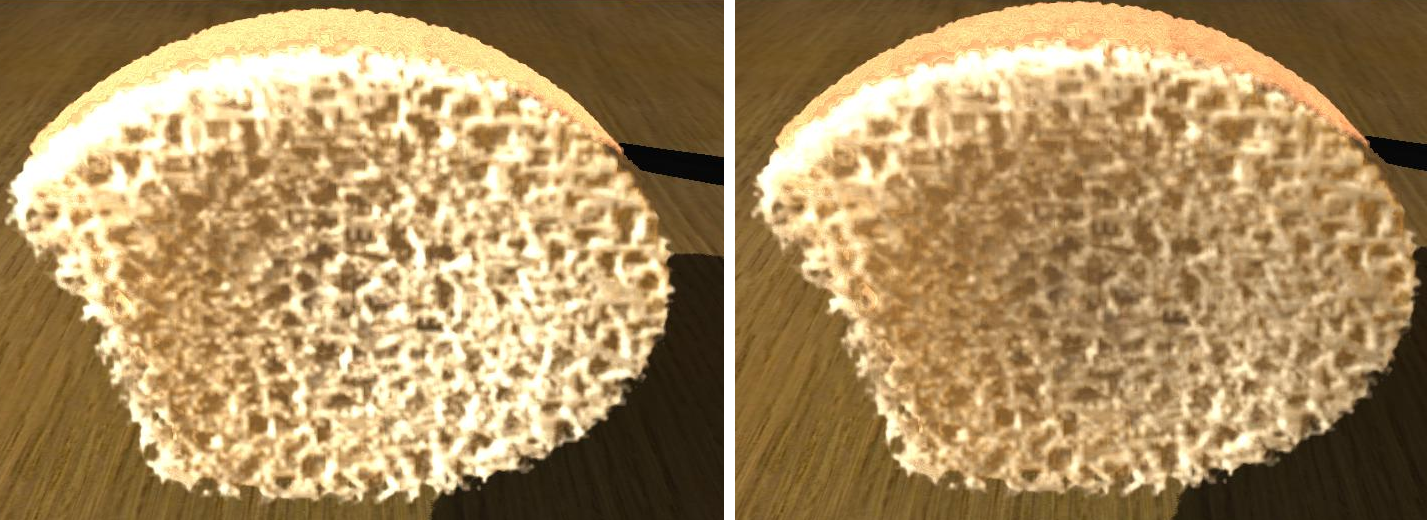
\includegraphics[width=13cm]{figures/occlusion}}
  \caption{Pan sin (izquierda) y con (derecha) oclusión de ambiente. La apariencia final se mejora notablemente, mostrando una apariencia natural.}
  \label{fg:occlusion}
\end{figure}
 
\subsection{Cómputo de las Normales}
Utilizamos un esquema {\em hacia adelante} en el cómputo de diferencias finitas del gradiente.
El gradiente en el punto será utilizado luego para computar la normal, la cual el vector diferencia normalizado, entre la posición {\em hacia adelante} y la posición actual del campo escalar,


\begin{equation}
\begin{aligned}
x &= tex(pos+(1,0,0)) - tex(pos)\\
y &= tex(pos+(0,1,0)) - tex(pos)\\
z &= tex(pos+(0,0,1)) - tex(pos) \\
N &= normalizar([x,y,z])
\end{aligned}
\end{equation}

Las normales y el vector que representa la luz permiten determinar la contribución especular en el punto, aplicando un modelo de Phong simple \cite{Phong1973}, y estableciendo un parámetro que permite al usuario especificar el impacto deseado para la componente especular.
Se han testeado otros modelos especulares más complejos, pero no se encontró diferencia apreciable en la apariencia final de la textura de pan.

\subsection{Cómputo de Sombras}
La técnica de DVR puede ser utilizada para computar sombreas realísticas, por medio de mapas de sombras \cite{Williams1978}.
Durante la generación del mapa de sombras, renderizamos muevamente un cubo representando el sistema de partículas.
El shader de fragmentos para ese cubo utiliza el mismo método de rayos explicado, pero solo computa la transmitancia en el rayo.
Si la transmitancia en ese rayo está por encima de un umbral al finalizar el cómputo, luego el fragmento no corresponde a un oclusor, y su profundidad se setea en infinito.
Si durante el cómputo de la transmitancia, la misma cae por debajo del umbral, la profundidad del fragmento se establece en la profundidad alcanzada por el rayo en ese momento.
Esta técnica se utiliza junto a un filtrado de porcentaje de cercanía, para generar sombras realísticas en nuestra aplicación.


\subsection{Corteza}
Es posible proveer al sistema con una función que indique si la posición es parte de la corteza o la miga, u otras consideraciones en otros materiales (por ejemplo, si el color de la sección de una esponja debe ser amarillo u verde).
Por ejemplo, una función puede definit una corteza cilíndrica asignando la etiqueta de miga a aquellas posiciones cercanas al eje del cilindro, y corteza a las restantes.
También se provee otra función que establece si la posición debe ser considerada aire.

Esto permite definir, de una manera intuitiva, la corteza y cortes en el volumen (ver Figs.~\ref{fg:crumb} y \ref{fg:results2}).

Los métodos para definir la misma fueron explica
dos en el capítulo anterior, utilizando un mapa de distancias o bien morfología matemática.


%%%%%%%%%%%%%%%

%Dentro del shader de fragmentos la primera operaci\'on es calcular la geometría de un rayo cuyo origen es la cámara de la escena y cuya dirección lo lleva hacia el fragmento siendo calculado. Este rayo es recorrido en intervalos regulares, evaluando la textura volumétrica para obtener la densidad del pan en esos puntos. Este valor se utiliza para calcular la transmitancia acumulada desde la cámara hasta el punto evaluado. Una vez que la transmitancia es menor que un valor preestablecido o el rayo sale del cubo que define el volumen, el cómputo termina.

%En cada punto evaluado también se computa la transmitancia dentro del volumen desde el punto hacia la fuente de luz en la escena. Esto se hace emitiendo un rayo desde el punto con dirección a la luz y nuevamente calculando la densidad en varios puntos del rayo. Con esta nueva información se aproxima la cantidad de luz que llega directamente al punto considerado, y permite representar sombras dentro del volumen.

%La información de transmitancia de los puntos evaluados del rayo principal y desde estos puntos hacia la luz se utilizan para calcular el color final del fragmento. A partir de esta información y tomando diferentes consideraciones artísticas pueden lograrse representaciones realísticas de diferentes materiales. En el caso de las imágenes de muestra presentadas en este trabajo el color del fragmento será más oscuro para areas del volumen que se consideran dentro de la corteza del pan y será de un color amarillo claro para la miga. También se usa un componente especular tenue. La información de transmitancia entre los puntos evaluados y la luz ayuda a proveer detalles de la estructura del pan. La Fig~\ref{fg:fragmentshader} muestra un esquema del cálculo del color final del pixel.

\section{Resultados}
Las imágenes obtenidas a partir del método descrito en la sección anterior fueron renderizadas en una computadora con una placa gráfica nVidia GTX 480 ($480$ cores), la cual es normalmente de uso hogareño.
La CPU fue una Intel(R) Core(TM) i5-2300 CPU (cuatro procesadores).
La resolución de las imágenes es de $1440\times990$ pixels. 

Se obtuvieron diferentes imágenes que semejan materiales horneados.
Diferentes tipos de pan pueden ser representados variando los parámetros de transmitancia y colores utilizados (ver Fig.~\ref{fg:fig5}).
En esa imagen mostramos panes donde no se aplica oclusión de ambiente.
En la imagen central los patrones producidos por los sistemas de partículas descritos en las secciones previas son claramente visibles.
En ese caso, el tiempo de vida de las partículas es diferente para cada una y de esa manera se obtienen burbujas de diferentes tamaños.

\begin{figure*}[htb!]
  \centerline{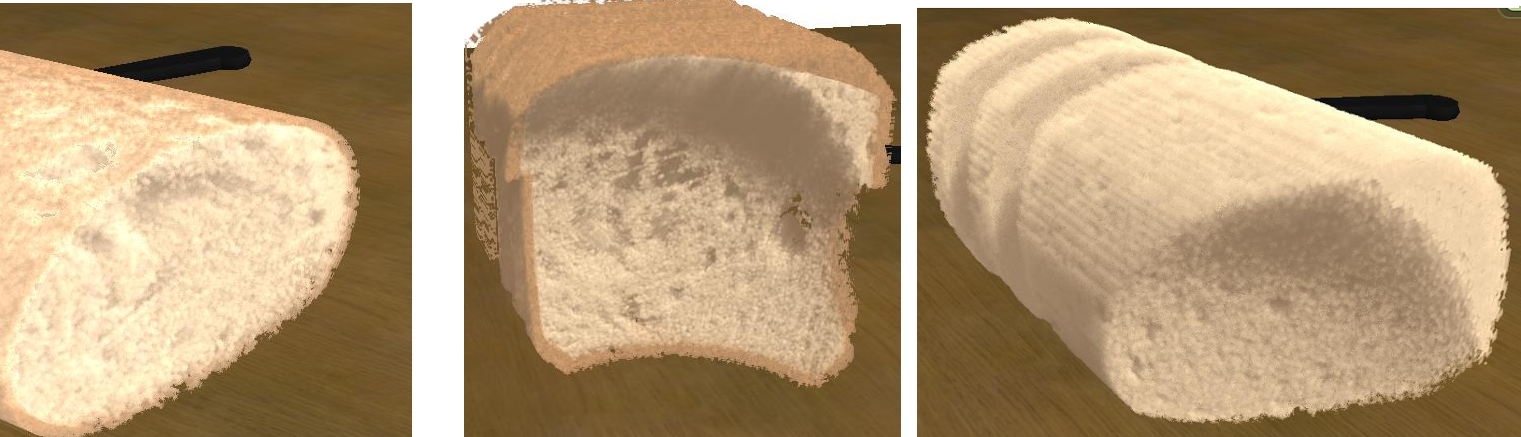
\includegraphics[width=13cm]{fig5}}
  \caption{Imágenes de diferentes tipos de pan renderizados en tiempo real, sin oclusión de ambiente. La imagen de la derecha muestra un pan sin corteza}
  \label{fg:fig5}
\end{figure*}

%La tabla muestra que los rayos secundarios constituyen el principal cuello de botella, lo cual es lógico, dado que a cada paso del rayo principal, el mismo computa un rayo secundario hacia la luz.


%\begin{table}[htb]
%\centering
%\begin{tabular}{|c|c|c|c|c|c|c|}
%\hline &  Pan 1 & Pan 2 & Pan 3 & Budín & Torta & Esponja \\
%\hline
%\hline
% FPS promedio  & 32.2 &  75.5 &  45.2 & 28.5 &  54.2 & 29.7\\
%\hline
% Puntos de evaluación &  140 &  140 &  140 & 256 &  140 & 256 \\
%\hline
% Transmitancia &  15 &  15 &  15 & 15 &  15 & 2.25 \\
%\hline
%\end{tabular}
%\caption{Tiempos de renderizado y parámetros de las imágenes de prueba.}
%\label{tab:n1}
%\end{table}

%\begin{table}[htb]
%\centering
%\begin{tabular}{|c|c|c|c|c|c|c|}
%\hline
% Pasos del rayo         & 128 &  256 \\
%\hline
%\hline
% Tiempo total shaders   & 10 ms &  32.5 ms \\
%\hline
% Rayo Principal         & 2 ms  & 5 ms  \\
%\hline
% Rayos Secundarios      &  8 ms & 27.5 ms  \\
%\hline
%\end{tabular}
%\caption{Detalle de tiempos de renderizado en milisegundos.}
%\label{tab:n2}
%\end{table}

La Fig.~\ref{fg:breads} muestra panes renderizados en tiempo real con oclusión de ambiente agregada.

\begin{figure*}[htb!]
  \centerline{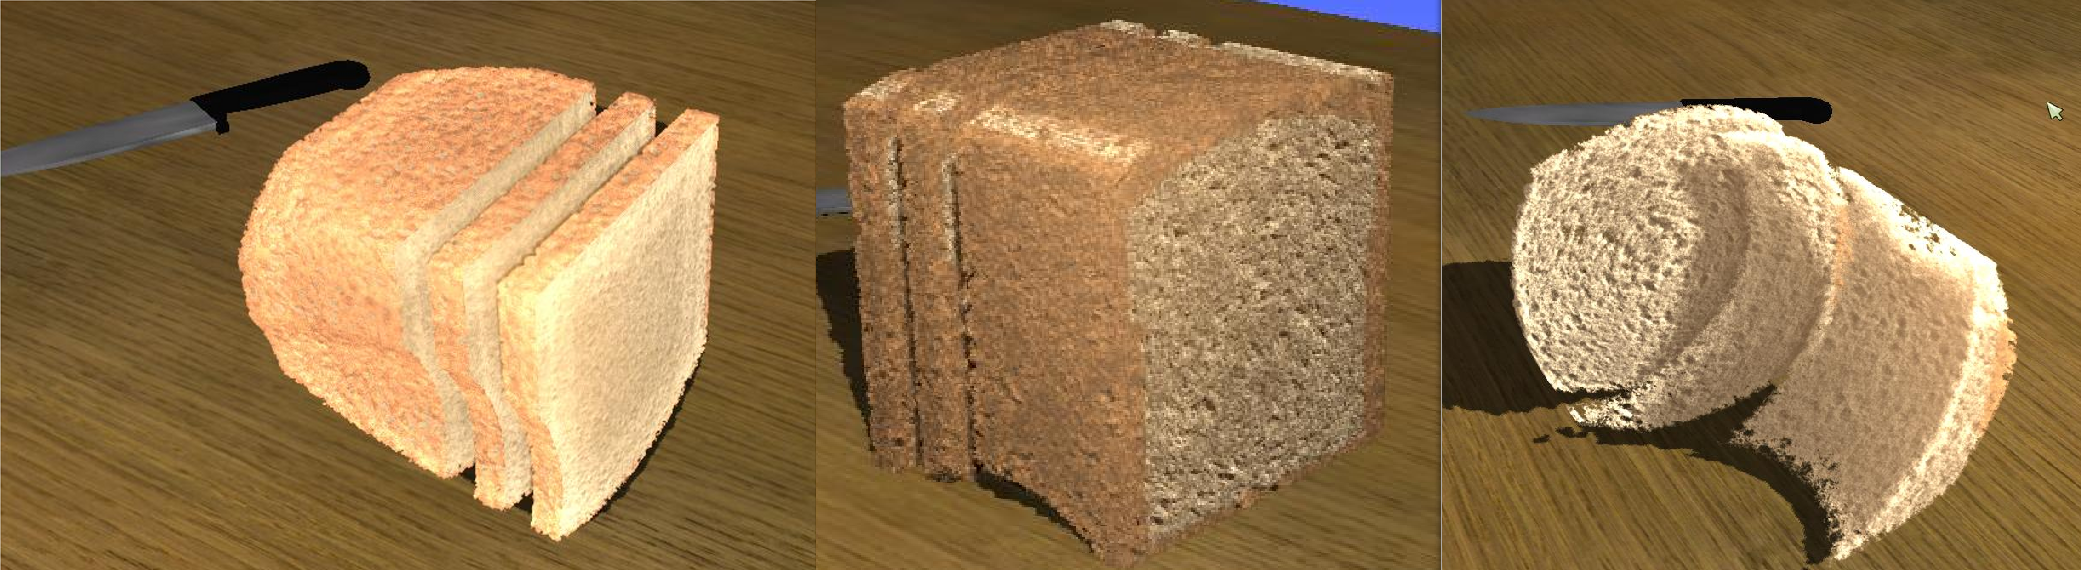
\includegraphics[width=13cm]{breads}}
  \caption{Imágenes de diferentes tipos de pan renderizados en tiempo real, con oclusión de ambiente.}
  \label{fg:breads}
\end{figure*}

Puede observarse que los panes con este efecto muestran un grado de realismo superior.

\subsection*{Tiempos de Cómputo}

Todas las imágenes fueron obtenidas en tasas de refresco de tiempo real (cuadros por segundo, FPS, por encima de $30$).
La eficiencia del proceso se resiente cuando la transmitancia es muy baja (el material es casi transparente), dado que se evaluarán más puntos en los rayos a recorrer antes de llegar al límite de transmitancia.
Otro parámetro importante es la cantidad de puntos a evaluar, ya que para cada paso computamos la transmitancia hacia la luz por medio de un rayo secundario.
Experimentalmente encontramos que utilizar $140$ o más pasos produce imágenes razonables para esponjas, pero se necesitan $300$ o más pasos para obtener imágenes razonables de panes, ver Fig.~\ref{fg:stepcount}.


\begin{figure}
  \centerline{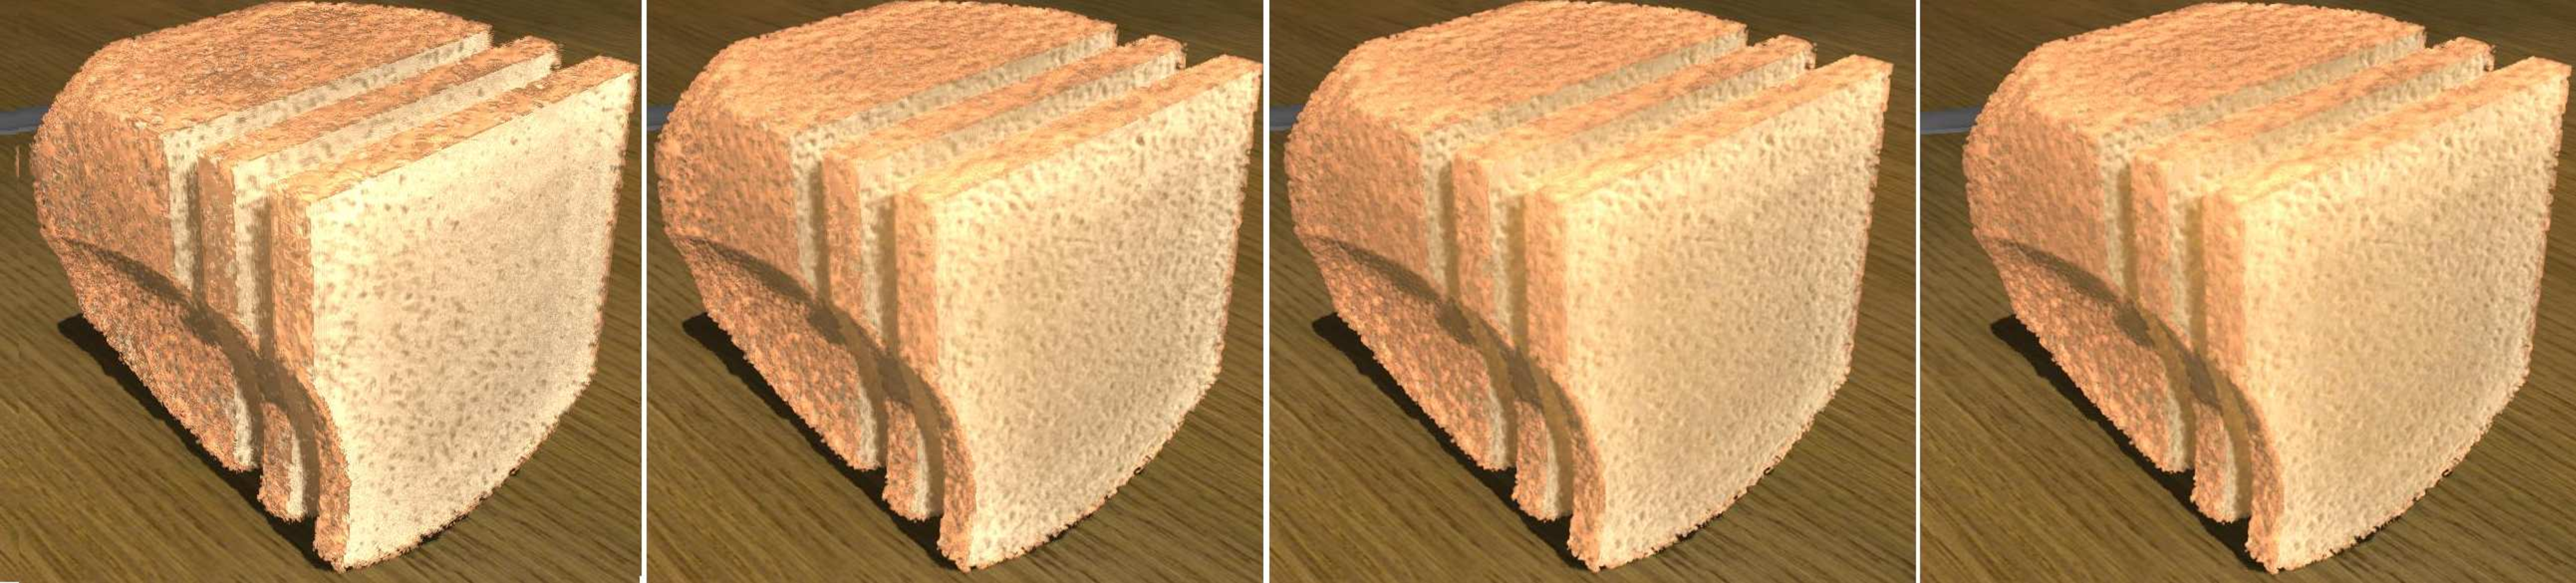
\includegraphics[width=13cm]{figures/stepcount}}
  \caption{Tiempos de cómputo de acuerdo a la cantidad de pasos utilizados. La imagen muestra que utilizar $300$ pasos del rayo produce imágenes razonables.}
  \label{fg:stepcount}
\end{figure}


En las regiones con corteza, la velocidad del método es mayor, ya que la transmitancia es menor para estas zonas, {\em i.e.}, los rayos necesitan menos pasos para alcanzar el umbral de opacidad que en regiones con mayor transmitancia.

\subsection{Otros Materiales y Efectos}
Es posible obtener otros materiales (ver Fig.~\ref{fg:fig6}).
Estos son el resultado de la variación de parámetros técnicos y artísticos del modelo.
En las imágenes de prueba pueden distinguirse un budín (izquierda), un pedazo de torta (medio) y una esponja (derecha).
En el caso de la esponja se modificaron los parámetros que definen la función de densidad.
Cuando no hay levadura en el proceso de creación puede utilizarse una textura volumétrica cuyos valores provienen de una función aleatoria.
En la Fig.~\ref{fg:sponges} puede observarse que la utilización de oclusión de ambiente produce imágenes de esponja más realistas que las obtenidas sin su aplicación.
La retroiluminación es también aproximada con este modelo (ver Fig.\ref{fg:fig7}).
En esa imagen puede apreciarse una esponja retroiluminada junto con la propagación de luz a través del volumen que representa.
Este efecto es una consecuencia natural del algoritmo volumétrico basado en RTE utilizado en este capítulo.

\begin{figure*}[htb!]
  \centerline{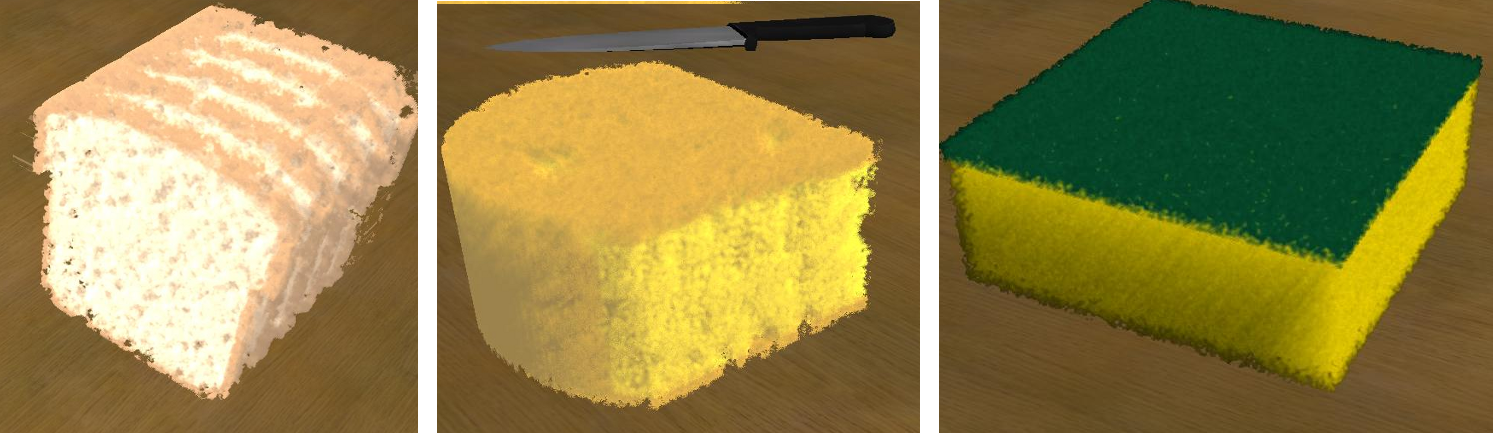
\includegraphics[width=13cm]{fig6}}
  \caption{Distintos materiales obtenidos a partir de diferentes configuraciones de parámetros. De izquierda a derecha: budín, torta y esponja. }
  \label{fg:fig6}

\end{figure*}

\begin{figure*}[htb!]
  \centerline{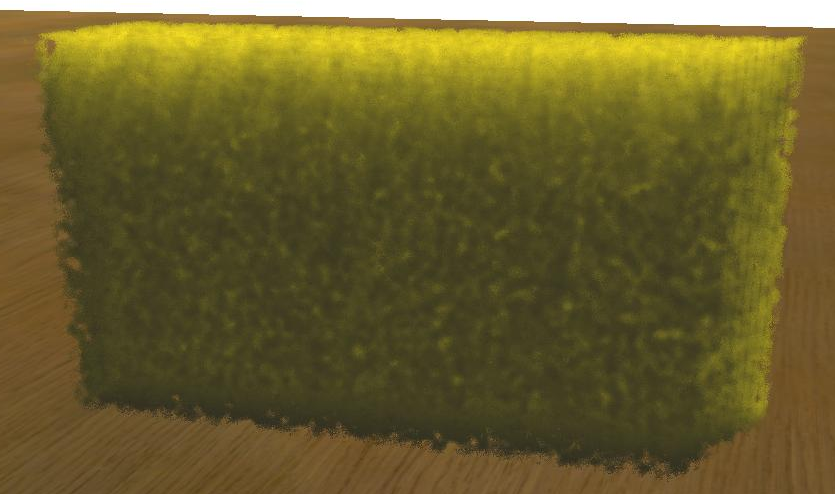
\includegraphics[width=8cm]{fig7}}
  \caption{Esponja retroiluminada.}
  \label{fg:fig7}
\end{figure*}


\begin{figure}
  \centerline{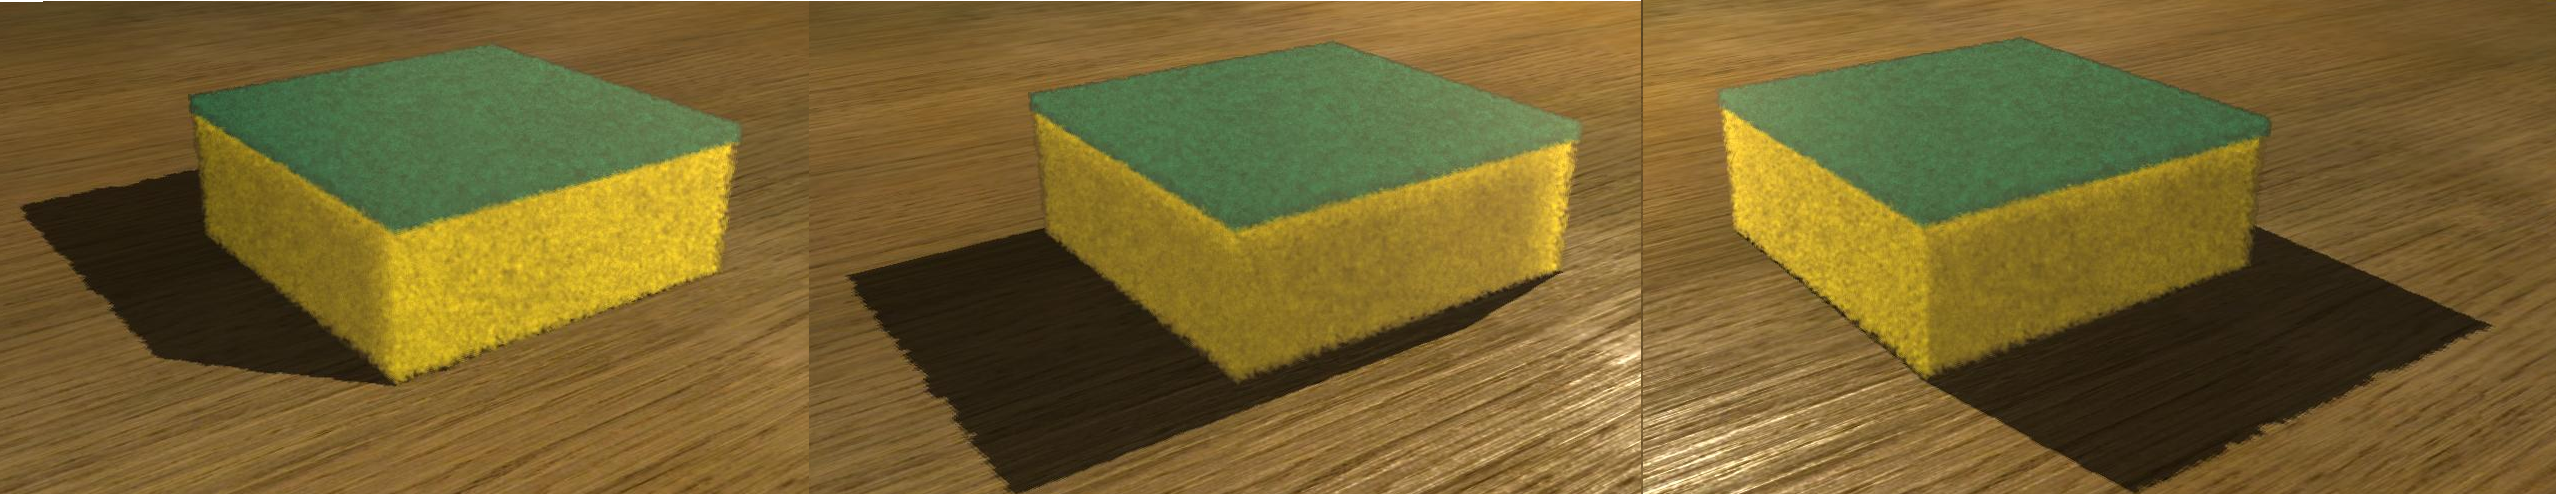
\includegraphics[width=13cm]{figures/sponges}}
  \caption{Esponjas renderizadas en tiempo real utilizando un campo escalar aleatorio como geometría, con oclusión de ambiente aplicada.}
  \label{fg:sponges}
\end{figure}

\section{Discusión}

%1)En primer lugar, un resumen de lo que hicimos en el paper y por qué es importante/novedoso

Hasta donde podemos ver en la literatura, en el tópico de renderizado de panes y otros materiales porosos, este es el primer trabajo que involucra tasas de refresco de tiempo real, sin la aparición de estructuras intermedias, procesos de captura onerosos, o post-procesamientos.

La literatura previa incluye pocos trabajos, como por ejemplo \cite{Cho2007}, pero las comparaciones con este método no son posibles, ya que los detalles claves del desarrollo no fueron explicados (tiempos de cómputo, método de renderización).
El método propuesto es compatible con el renderizado de ráster en tiempo real disponible en las GPUs actuales, contando con la capacidad de producir un material realista.
El método puede ser integrado con facilidad en cualquier motor $3D$ basado en shaders.
Además, la técnica de mapeo de sombras permite integrar el material en escenas de una manera natural.

%3) Recordamos que las imagenes obtenidas fueron buenas, y que obtuvimos otros materiales cambiando pocos parametros

El algoritmo de renderizado es lo suficientemente flexible como para modelar diferentes materiales, como pan, esponjas, y tortas, cambiando unos pocos parámetros.
Otros materiales porosos como pizzas, quesos, y otros, pueden ser fácilmente obtenidos definiendo geometrías adecuadas y parámetros de transmitancia y cantidad de pasos.
Es decir, se pueden obtener diversos materiales con el mismo método.

Además, nuestra representación volumétrica permite realizar cortes en tiempo real en la miga y corteza del pan.
Esto puede resultar de gran ayuda en diversas aplicaciones, entre las cuales encontramos video juegos.

Respecto al modelo de iluminación, el éxito visual obtenido por el método a la hora de obtener una apariencia que semeja al pan en tiempo real, parece estar dado por la utilización de oclusión ambiente, además de los agregados discutidos sobre el algoritmo básico de DVR.

Debemos destacar que el mayor incremento en el realismo final en las imágenes fue dado a la inclusión del término de oclusión de ambiente, el cual proporcionó una textura mucho más detallada, mostrando una mayor complejidad y riqueza subyacente.
Otros efectos que introdujimos, como el reflejo especular de Phong, también incidieron sobre el realismo final.
Sin embargo, métodos especulares más sofisticados (por ejemplo, el modelo de Cook-Torrance \cite{Cook1982}) no mejoraron de manera apreciable las imágenes.

%5)Tiempos de cómputo (muy importante en este paper!)

Los tiempos de cómputo alanzados fueron adecuados para alcanzar tiempo real en computadoras estándares al año de publicación de la presente tesis (utilizamos una placa de video nVidia GTX 480, junto con una CPU Intel(R) i5).

En la gran mayoría de los casos, las tasas de refresco alzancadas fueron de tiempo real.
Los únicos casos que no lograron dichos tiempos ocurrieron cuando el objeto a ser renderizado ocupó una porción bastante considerable de la pantalla, ya que el método está implementado en el shader de fragmentos.
Los tiempos de cómputo finales dependen de la cantidad de pasos utilizados y el coeficiente de transmitancia.

Adicionalmente, diferentes materiales cuentan con diferentes tiempos de cómputo para su renderización.
Por ejemplo, un tiempo de cómputo adecuado para simular esponjas es más bajo que aquél que se necesita para modelar migas de panes.
Esto puede atribuirse al hecho de que el método necesita más pasos para capturar las burbujas macroscópicas del pan.

Las GPUs actuales poseen límites en las texturas volumétricas que pueden soportar.
Esto limita la calidad de las imágenes que podemos obtener, ya que a mayor resolución, fue demostrado que puede obtenerse un mayor detalle y realismo en las imágenes.
Por lo tanto, las aplicaciones en tiempo real deben limitar la resolución de la textura que se carga en la GPU.
En otras palabras, acercamientos extremos a la estructura a ser renderizada puede dar lugar áreas homogéneas (sin detalle).
Esta limitación está atada al tamaño de textura de la GPU, y será eventualmente superado con la mejora del hardware de la próxima generación de GPUs.
En aplicaciones fuera de línea, es posible utilizar texturas lo suficientemente grandes que dan lugar a imágenes foto-reaísticas.

\section{Conclusiones}

En este capítulo hemos aplicado el modelo de transmitancia del renderizado directo de volúmenes utilizando la GPU, sobre un campo escalar tridimensional representando la estructura de la miga del pan (la cual fue computada en el capítulo anterior).
Se obtuvieron imágenes realistas en tiempo real.
Debido a limitaciones del hardware, también se obtuvieron imágenes con aún mayor detalle, pero a tasas de refresco menores.

El algoritmo presentado fue implementado en el shader de fragmento utilizando componentes especulares y difusas, cómputo de normales y oclusión de ambiente.

Los resultados alcanzados superan en gran medida al estado del arte, obteniendo imágenes que simulan el material en tiempo real con gran realismo.
El método presenta aplicaciones en diversas áreas, como video juegos, juegos serios \cite{Susi2007} y renderizado foto-realista.

Estas técnicas son mucho más simples y no presentan las desventajas de otros métodos, como procesos de captura, generación de mallas o post-procesos.

Estos resultados demuestran que la elección de una representación volumétrica es la adecuada para estos materiales porosos.



